\section{Minimalizacja w 1-D}
  \begin{frame}{Minimalizacja w 1-D}
    \begin{block}{Przydatność metod 1-D dla zag. n-D}
      \begin{itemize}
        \item prosta ilustracja ogólnych problemów
        \item metody 1-D -- często: element składowy metod n-D

      \end{itemize}

    \end{block}

  \end{frame}

\subsection{Przeglądanie siatki (grid search)}
  \begin{frame}{Przeglądanie siatki \emph{(grid search)}}
    % \centering
    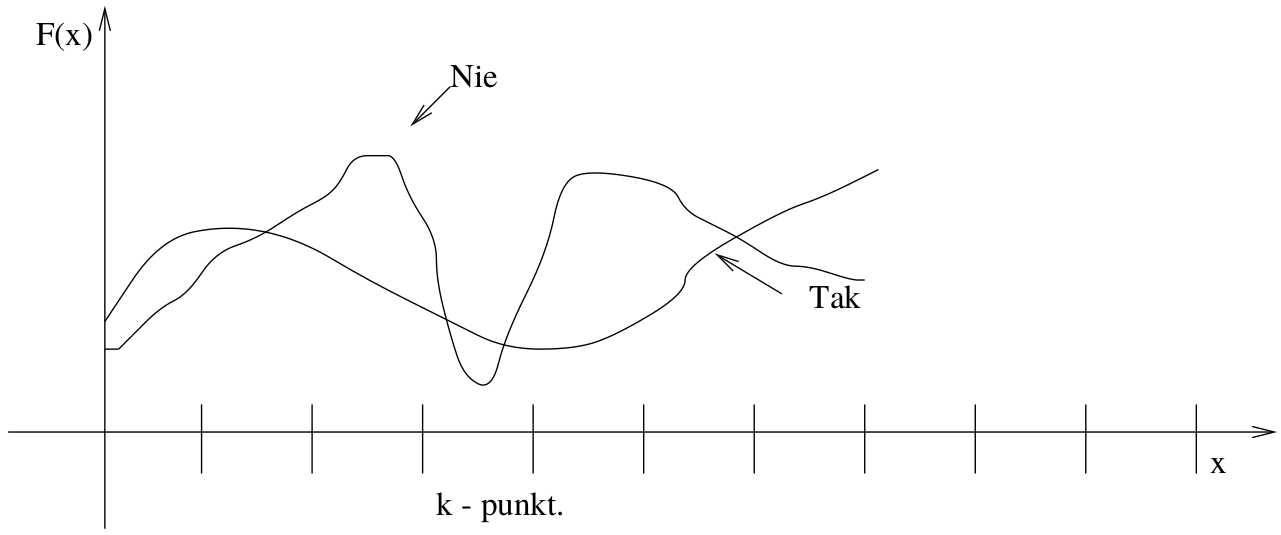
\includegraphics[width=1\textwidth]{img/17/przegladanie_siatki}
  \end{frame}
